%-----------------------
%	CONFIGURATIONS
%-----------------------

\documentclass[12pt,a4paper,oneside]{article}

\usepackage[utf8]{inputenc}
\usepackage[colorlinks=true, citecolor=blue, linkcolor=black]{hyperref}
\usepackage{graphicx}
% \usepackage{natbiba}
\usepackage{tabu}
\usepackage{multirow}
\usepackage{amsmath}
\usepackage{amsthm}
\usepackage{caption}
\usepackage{subcaption}
\usepackage{tikz}
\usetikzlibrary{positioning,arrows,shapes}
\graphicspath{ {images/} }
\usepackage[a4paper,left=2cm,right=2cm,top=2.5cm,bottom=2.5cm]{geometry}
\setcounter{section}{-1}

\theoremstyle{definition}
\newtheorem{exmp}{Example}[section]

\newtheorem{theorem}{Theorem}[section]

%-----------------------
%	INFORMATION
%-----------------------

\title{Tópicos Avançados em Algoritmos (TAA) - Practical Assignment 2 \\\large Implementing AVL and Red-Black Trees}

\author{João Rebelo Pires\footnote{João Rebelo Pires - 201200384}}

\date{DCC - FCUP, May 2017}

\begin{document}

\maketitle

%-----------------------
%	SECTION 0
%-----------------------

\section{How To}\label{sec:for_dummies}

In this section, we simply want to explain how to compile and execute our implementation.

First of all, we have to notice that we have two different folders under folder \texttt{src}:

\begin{itemize}
	\item \texttt{avl};
	\item \texttt{rbt}.
\end{itemize}

The first folder has our implementation for AVL trees, and the second one has our implementation for Red-Black trees.

The input and output description, as well as compilation and execution instructions are the same, assuming you are in the correct folder.

% Subsection 1
\subsection{Input Description}\label{subsec:input_descrip}

For simple tests, we can assume that we have a set of integers we want to give to our implementation. With that in mind, the input consists of a number, $n$, followed by $n$ lines each with an integer.

% Subsection 2
\subsection{Output Description}\label{subsec:output_descrip}

The output consists of $6$ lines. The first, describes how much time in milliseconds it took our implementation to insert every number in the tree. The second and the forth print the minimum and maximum values, respectively, in our tree, while the third and fifth print the time in milliseconds it took to find these values. Finally, the last line prints the time in milliseconds it took our implementation to delete every node, one by one, from our tree, in the order they were inserted, to test the complexity of the deletion function.

% Subsection 3
\subsection{Compilation}\label{subsec:compile}

Our implementation is compiled differently if you are in \textit{Linux} or in \textit{MacOS X}. However, that is handled by the \texttt{Makefile} file.

With that in mind, all you have to do to compile is run the following line:

\texttt{make} or \texttt{make all}.

In order to clean everything after executing, simply run the following line:

\texttt{make clean}.

% Subsection 4
\subsection{Execution}

The compiler generates an executable named \textbf{main}. To execute it, simply execute the following command line:

\texttt{./main}.\\

If you have an input file \textbf{test.in}, you should execute the following command line instead:

\texttt{./main < test.in}.

%-----------------------
%	SECTION 1
%-----------------------
\section{Introduction}\label{sec:intro}
For this assignment we had the task of implementing two data structures from a list given. 

The algorithm presented implements Red-Black Trees and AVL Trees, in \texttt{C++}.

For Red-Black Trees, there is also a simple and small implementation of iterators, with simple functions that are also implemented in STL implementation for sets, but that are not guaranteed to be functioning efficiently.

%-----------------------
%	SECTION 2
%-----------------------
\section{Balanced Binary Search Trees}

In this section, we will simply define some concepts about Balanced Binary Search Trees.

% Subsection 1
\subsection{Binary Search Trees}\label{subsec:bst}

A \textbf{Binary Search Tree} (BST) is a rooted binary tree (rooted here simply means that the root is established as being the root). Every node in a BST stores a key (that can be an \texttt{int}, a \texttt{string}, etc.) and two distinguished sub-trees, commonly denoted \textbf{left} and \textbf{right}. It also stores the information about its \textbf{parent} (which for the root is none).

The tree additionally satisfies the binary search tree property, which states that the key in each node must be greater than any key stored in the left sub-tree, and less than any key stored in the right sub-tree.
 
One of the major advantages of BSTs over other data structures is that it is very efficient to get the elements by order.

% Subsection 2
\subsection{Self-balancing BSTs}\label{subsec:sb-BST}
In the previous subsection we have defined what a BST is.

If we analyse the complexity of the operations defined in BST (like \textbf{insert}, \textbf{delete}, \textbf{search}, we can see that if the tree has height $h$, then this complexity is $\mathcal{O} \left( h \right)$ time. Thus, these operations are fast if the height of the seearch tree is small. If its height is large, however, the operations may run no faster than with a linked list.

A self-balancing BST is a type of BST that, from time to time, changes somehow the tree in order to maintain a property that makes sure the tree is always balanced according to some criteria.

In this work, we discuss two types of self-balancing trees. In Section \ref{sec:rb-trees} we discuss Red-Black trees and in Section \ref{sec:avl-trees}.


%-----------------------
%	SECTION 3
%-----------------------
\section{Red-Black Trees}\label{sec:rb-trees}
A \textbf{Red-Black tree} is a BST with one extra information about each node: its \textbf{color}, which can be either \texttt{RED} or \texttt{BLACK}.

A Red-Black tree is a a BST that satisfies the following \textbf{red-black properties}:

\begin{enumerate}
	\item Every node is either red or black;
	\item The root is black;
	\item Every leaf is black;
	\item If a node is red, then both its children are black;
	\item For each node, all simple paths from the node to descendant leaves contain the same number of black nodes.
\end{enumerate}

An example of a Red-Black tree is in Figure \ref{fig:rbt-ex1}.

The number of black nodes in the path from a node to their leaves (not including the node itself) is called \textbf{black height} and it can be written as $bh \left( n \right)$.

\begin{figure}
\centering
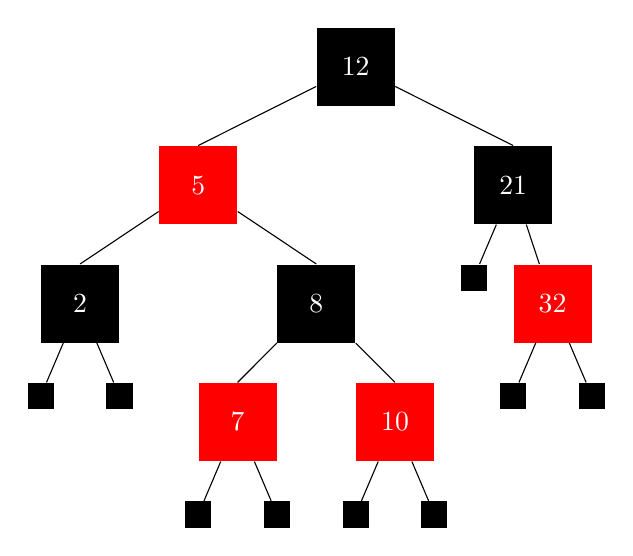
\begin{tikzpicture}[
	leaf/.style={regular polygon, regular polygon sides=4, draw=none, fill=black, text centered, anchor=north, text=white},
	blackn/.style={regular polygon, regular polygon sides=4, draw=none, fill=black, text centered, anchor=north, text=white, minimum size = 1.4cm},
    redn/.style={regular polygon, regular polygon sides=4, draw=none, fill=red, text centered, anchor=north, text=white, minimum size = 1.4cm},
    level distance=0.5cm, growth parent anchor=south]
    
    \node (root) [blackn] {$12$} [-]
    	[sibling distance=4cm]
    	child {
    		[sibling distance=3cm]
    		node (child1) [redn] {$5$}
    		child {
    			[sibling distance=1cm]
    			node (child7) [blackn] {$2$}
    			child { node (child8) [leaf] { } }
    			child { node (child9) [leaf] { } }
    		}
    		child {
    			[sibling distance=2cm]
    			node (child10) [blackn] {$8$}
    			child {
    				[sibling distance=1cm]
    				node (child11) [redn] { $7$ }
    				child { node (child12) [leaf] { } }
    				child { node (child13) [leaf] { } }
    			}
    			child {
    				[sibling distance=1cm]
    				node (child14) [redn] { $10$ }
    				child { node (child15) [leaf] { } }
    				child { node (child16) [leaf] { } }
    			}
    		}
    	}
    	child {
    		[sibling distance=1cm]
    		node (child2) [blackn] {$21$}
    		child { node (child3) [leaf] { } }
    		child {
    			node (child4) [redn] { $32$ }
    			child { node (child5) [leaf] { } }
    			child { node (child6) [leaf] { } }
    		}
    	};

\end{tikzpicture}
\caption{Example of a Red-Black tree.}\label{fig:rbt-ex1}
\end{figure}

\begin{exmp}
In Figure \ref{fig:rbt-ex1}, we have the following black heights:

\begin{itemize}
	\item $bh \left( 12 \right) = 2$;
	\item $bh \left( 21 \right) = 1$;
	\item $bh \left( 5 \right) = 2$.
\end{itemize}
\end{exmp}

The important now is to see what kind of balance do these properties guarantee.

We note that if $bh \left( n \right) = k$, then a path from node $n$ to descendant leaves has at least $k$ nodes (all black) and at most $2k$ nodes (red and black, alternating - a red node can not have a red child).

Thus, the following theorem holds.

\begin{theorem}[Height of a Red-Black Tree]\label{th:rb-height}
	A Red-Black tree with $n$ nodes has at most height $2 \times \log _{2} \left( n + 1 \right)$.
	
	This means that the height of a Red-Black tree is $\mathcal{O} \left( \log n \right)$. \\
\end{theorem}

How to insert a node in a non empty Red-Black tree?

First of all, \textbf{insert} the node as in any other BST. \textbf{Color} the node as \textbf{red} (adding the "null" children). Recolor and restructure if necessary, in order to restore the properties.

With this three steps, we guarantee that the only property that can be violated property 4. If the parent of the node we inserted now is black, we don't need to do anything. If it is red, the following may happen (assuming $z$ is the node inserted now):

\begin{itemize}
	\item \textbf{Case 1:} $z$'s uncle $y$ is red;
	\item \textbf{Case 2:} $z$'s uncle $y$ is black and $z$ is a right child;
	\item \textbf{Case 3:} $z$'s uncle $y$ is black and $z$ is a left child.
\end{itemize}

Each case is handled differently.

The same happens while deleting a node, that is, a series of cases may arise that are handled differently. The idea is a bit more complicated than when inserting, but the first thing we have to do is similar to deleting a node in a regular BST. The following cases may arise:

\begin{itemize}
	\item \textbf{Case 1:} $x$'s sibling $w$ is red;
	\item \textbf{Case 2:} $x$'s sibling $w$ is black and both of $w$'s children are black;
	\item \textbf{Case 3:} $x$'s sibling $w$ is black, $w$'s left child is red, and $w$'s right child is black;
	\item \textbf{Case 4:} $x$'s sibling $w$ is black, and $w$'s right child is red.
\end{itemize}


% Subsection 1
\subsection{Implementation and Complexity}\label{subsec:rb-impl}

Since the code is well commented, this subsection will mostly discuss the complexity associated with each method.

From Theorem \ref{th:rb-height} we can see that \texttt{insert}, \texttt{erase}, \texttt{find}, \texttt{minValue} and \texttt{maxValue} all take $\mathcal{O} \left( \log n \right)$ time.

Since \texttt{size} only returns the value of a globally declared variable, it takes $\mathcal{O} \left( 1 \right)$ time. On the other hand, since \texttt{empty} only verifies if \texttt{size} is $0$, it also takes $\mathcal{O} \left( 1 \right)$ time.

% Subsection 1
\subsection{Testing Complexity and Complexity Verification}\label{subsec:rb-tst}

Since we have $n$ insertions, the whole complexity expected is $\mathcal{O} \left( n \log n \right)$. With that in mind, we can see in Table \ref{tab:rbt-tbl} that the results for insertions are as expected.

Imagine you have a test with input size $n$ that runs in $t$ seconds. If you run a test with input size $10 \times n$, this new test is expected to run in something in the order of $10 \times \log \left( n \right) \times t$ seconds. This is consistent with the results.

\begin{table}[h!]
\centering
\begin{tabular}{c|c|c|c|c|c|c|}
\cline{2-7}
& \multicolumn{6}{ c| }{Test File Number} \\ \cline{2-7}
& 1 & 2 & 3 & 4 & 5 & 6 \\ \cline{1-7}
\multicolumn{1}{ |c| }{Size of Input ($n$)} & 10000000 & 10000000 & 1000000 & 1000000 & 100000 & 100000 \\ \cline{1-7}
\multicolumn{1}{ |c| }{Time (seconds)} & 45.5767 & 45.2978 & 3.65674 & 3.66747 & 0.289648 & 0.296571 \\ \cline{1-7}
%\multicolumn{1}{ |c| }{$\log n$} & 23.2534 & 23.2534 & 19.9315 & 19.93156 & 16.6096 & 16.6096 \\ \cline{1-7}

\end{tabular}
\caption{Results for the insertion tests to our Red-Black tree.}\label{tab:rbt-itbl}
\end{table}

Table \ref{tab:rbt-rtbl}, on the other hand, shows the results for deletion. The expected time complexity is also $\mathcal{O} \left( n \log n \right)$, for the same reason as for insertion.

The results were also what we expected.

\begin{table}[h!]
\centering
\begin{tabular}{c|c|c|c|c|c|c|}
\cline{2-7}
& \multicolumn{6}{ c| }{Test File Number} \\ \cline{2-7}
& 1 & 2 & 3 & 4 & 5 & 6 \\ \cline{1-7}
\multicolumn{1}{ |c| }{Size of Input ($n$)} & 10000000 & 10000000 & 1000000 & 1000000 & 100000 & 100000 \\ \cline{1-7}
\multicolumn{1}{ |c| }{Time (seconds)} & 18314.2 & 18.8544 & 1.48907 & 1.2611 & 0.074103 & 0.07522 \\ \cline{1-7}
%\multicolumn{1}{ |c| }{$\log n$} & 23.2534 & 23.2534 & 19.9315 & 19.93156 & 16.6096 & 16.6096 \\ \cline{1-7}

\end{tabular}
\caption{Results for the deletion tests to our Red-Black tree.}\label{tab:rbt-rtbl}
\end{table}

Finally, we can also analyse the complexity for the minimum and maximum values in our tree. Table \ref{tab:rbt-minmaxtbl} shows that these functions are really fast.


\begin{table}[h!]
\centering
\begin{tabular}{c|c|c|c|c|c|c|}
\cline{2-7}
& \multicolumn{6}{ c| }{Test File Number} \\ \cline{2-7}
& 1 & 2 & 3 & 4 & 5 & 6 \\ \cline{1-7}
\multicolumn{1}{ |c| }{Size of Input ($n$)} & 10000000 & 10000000 & 1000000 & 1000000 & 100000 & 100000 \\ \cline{1-7}
\multicolumn{1}{ |c| }{Time min (milliseconds)} & 0.008 & 0.006 & 0.004 & 0.005 & 0.005 & 0.004 \\ \cline{1-7}
\multicolumn{1}{ |c| }{Time max (milliseconds)} & 0.005 & 0.004 & 0.003 & 0.003 & 0.003 & 0.002 \\ \cline{1-7}
%\multicolumn{1}{ |c| }{$\log n$} & 23.2534 & 23.2534 & 19.9315 & 19.93156 & 16.6096 & 16.6096 \\ \cline{1-7}

\end{tabular}
\caption{Results for the minimum and maximum tests to our Red-Black tree.}\label{tab:rbt-minmaxtbl}
\end{table}

%-----------------------
%	SECTION 4
%-----------------------
\section{AVL (G. \underline{A}delson-\underline{V}elsky e E. \underline{L}andis) Trees}\label{sec:avl-trees}

From Theorem \ref{th:rb-height} in Section \ref{sec:rb-trees} we saw that the majorant for the height of a Red-Black tree with $n$ nodes is $2 \times \log _{2} \left( n + 1 \right)$. AVL trees are a kind of self-balancing trees that have the following property:

For each node in an AVL tree, the height of the left subtree and the height of the right subtree differ at most by $1$.

With that in mind, each node will not have a bit with its color, but rather an integer representing its height. The height of a node is $1$ unit more than the maximum between the heights of its two children. The height of a leaf is defined to be $0$, and since a leaf has both his left and right child being \textit{null}, it is convenient to define that the height of a \textit{null} node is $-1$.

% Subsection 1
\subsection{Testing Complexity and Complexity Verification}\label{subsec:avl-tst}

Since we have $n$ insertions, the whole complexity expected is $\mathcal{O} \left( n \log n \right)$. With that in mind, we can see in Table \ref{tab:avl-itbl} that the results for insertions are as expected.

\begin{table}[h!]
\centering
\begin{tabular}{c|c|c|c|c|c|c|}
\cline{2-7}
& \multicolumn{6}{ c| }{Test File Number} \\ \cline{2-7}
& 1 & 2 & 3 & 4 & 5 & 6 \\ \cline{1-7}
\multicolumn{1}{ |c| }{Size of Input ($n$)} & 10000000 & 10000000 & 1000000 & 1000000 & 100000 & 100000 \\ \cline{1-7}
\multicolumn{1}{ |c| }{Time (seconds)} & 51.9432 & 53.1062 & 4.13072 & 4.11807 & 0.329399 & 0.338172 \\ \cline{1-7}
%\multicolumn{1}{ |c| }{$\log n$} & 23.2534 & 23.2534 & 19.9315 & 19.93156 & 16.6096 & 16.6096 \\ \cline{1-7}

\end{tabular}
\caption{Results for the insertion tests to our AVL tree.}\label{tab:avl-itbl}
\end{table}

As for deletion, an error was discovered while testing for these huge sets of data, which was not discovered while testing with small cases. First, deletion was not working if we were deleting the root of the tree, giving \texttt{Segmentation fault}. After that was solved, another error was yet discovered, and after a lot of debug, I was able to discover where the error was located (the function \texttt{rotate} has an error that seems to only give problems with deletion) that I was, unfortunately, unable to fix.

Finally, we can also analyse the complexity for the minimum and maximum values in our tree. Table \ref{tab:avl-minmaxtbl} shows that these functions are really fast.


\begin{table}[h!]
\centering
\begin{tabular}{c|c|c|c|c|c|c|}
\cline{2-7}
& \multicolumn{6}{ c| }{Test File Number} \\ \cline{2-7}
& 1 & 2 & 3 & 4 & 5 & 6 \\ \cline{1-7}
\multicolumn{1}{ |c| }{Size of Input ($n$)} & 10000000 & 10000000 & 1000000 & 1000000 & 100000 & 100000 \\ \cline{1-7}
\multicolumn{1}{ |c| }{Time min (milliseconds)} & 0.009 & 0.007 & 0.005 & 0.004 & 0.004 & 0.004 \\ \cline{1-7}
\multicolumn{1}{ |c| }{Time max (milliseconds)} & 0.005 & 0.004 & 0.003 & 0.003 & 0.003 & 0.002 \\ \cline{1-7}
%\multicolumn{1}{ |c| }{$\log n$} & 23.2534 & 23.2534 & 19.9315 & 19.93156 & 16.6096 & 16.6096 \\ \cline{1-7}

\end{tabular}
\caption{Results for the minimum and maximum tests to our AVL tree.}\label{tab:avl-minmaxtbl}
\end{table}

%-----------------------
%	SECTION 5
%-----------------------

\section{Input Tests and Final Remarks}\label{sec:input_final}

The input tests used are the files with the name \texttt{tst[1-6].in}.

Since find is really fast, we were not able to verify that finding an element in an AVL tree is faster than finding an element in a Red-Black tree (which would be a trivial observation, since the maximum height of an AVL tree is less than the maximum height of a Red-Black tree). Even so, we can verify by comparison between Table \ref{tab:rbt-itbl} and Table \ref{tab:avl-itbl} that it is indeed faster to insert in a Red-Black tree than in an AVL tree, which is what we expected.

There is a commented section in file \texttt{rbt.cpp} where one can test the implementation of the iterators.

\end{document}
